\documentclass[border=4pt]{standalone}
\usepackage{amsmath,amssymb}
\usepackage{tikz}
\usetikzlibrary{arrows.meta,shadows}
\begin{document}
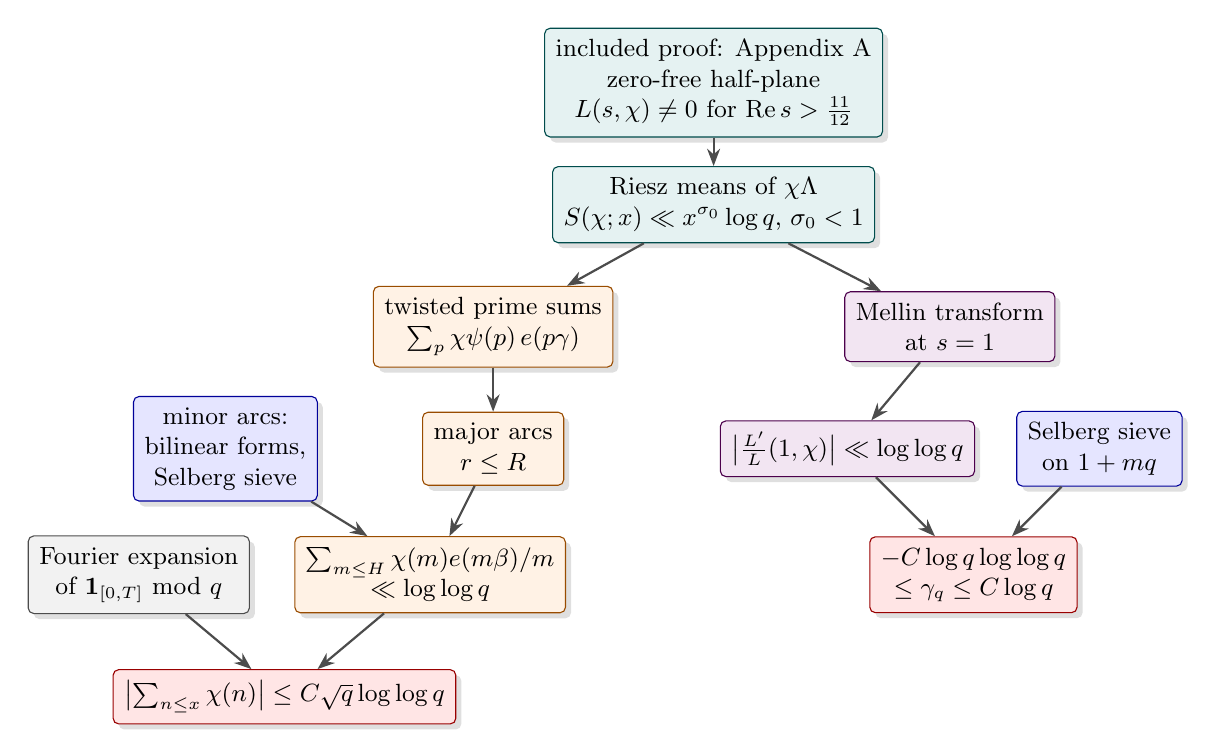
\begin{tikzpicture}[
  box/.style={draw=#1!60!black,fill=#1!10,rounded corners=2pt,align=center,
              font=\small,inner sep=4pt,drop shadow={opacity=0.25,shadow xshift=2pt,shadow yshift=-2pt}},
  >={Stealth[length=2.2mm]}, arr/.style={->,thick,gray!60!black}]
  \node[box=teal] (hp) at (1.2,0) {included proof: Appendix A\\zero-free half-plane\\$L(s,\chi)\neq0$ for $\operatorname{Re}s>\frac{11}{12}$};
  \node[box=teal] (rz) at (1.2,-1.55) {Riesz means of $\chi\Lambda$\\$S(\chi;x)\ll x^{\sigma_0}\log q$, $\sigma_0<1$};
  \node[box=orange] (tw) at (-1.6,-3.1) {twisted prime sums\\$\sum_p\chi\psi(p)\,e(p\gamma)$};
  \node[box=violet] (me) at (4.2,-3.1) {Mellin transform\\at $s=1$};
  \node[box=blue] (mi) at (-5.0,-4.65) {minor arcs:\\bilinear forms,\\Selberg sieve};
  \node[box=orange] (ma) at (-1.6,-4.65) {major arcs\\$r\le R$};
  \node[box=violet] (ld) at (2.9,-4.65) {$\bigl|\frac{L'}L(1,\chi)\bigr|\ll\log\log q$};
  \node[box=blue] (bs) at (6.1,-4.65) {Selberg sieve\\on $1+mq$};
  \node[box=gray] (po) at (-6.1,-6.25) {Fourier expansion\\of $\mathbf 1_{[0,T]}$ mod $q$};
  \node[box=orange] (hs) at (-2.4,-6.25) {$\sum_{m\le H}\chi(m)e(m\beta)/m$\\$\ll\log\log q$};
  \node[box=red] (ek) at (4.5,-6.25) {$-C\log q\log\log q$\\$\le\gamma_q\le C\log q$};
  \node[box=red] (pv) at (-4.25,-7.8) {$\bigl|\sum_{n\le x}\chi(n)\bigr|\le C\sqrt q\log\log q$};
  \draw[arr] (hp)--(rz);
  \draw[arr] (rz)--(tw);
  \draw[arr] (rz)--(me);
  \draw[arr] (tw)--(ma);
  \draw[arr] (ma)--(hs);
  \draw[arr] (mi)--(hs);
  \draw[arr] (hs)--(pv);
  \draw[arr] (po)--(pv);
  \draw[arr] (me)--(ld);
  \draw[arr] (ld)--(ek);
  \draw[arr] (bs)--(ek);
\end{tikzpicture}
\end{document}
